\documentclass{article}
\usepackage[utf8]{inputenc}
\usepackage{setspace}
\usepackage{tabto}
\usepackage{graphicx}

\title{A Brief History on Mobile Apps and Their Market Impact}
\author{Payton Lo}
\date{May 2022}

\doublespacing
\begin{document}

\maketitle

\section{Abstract}
\tab This paper analyzes the birth and development of mobile applications, starting with the impact of IBM's SIMON. After examining these early prototypes it shifts to development from 2001 to around 2010, looking at Symbian and BlackBerryOS, the market leaders at the time. In the early 2010's, Symbian and BlackBerryOS's market share dwindled. This paper examines the differences between the two, why they both ended up failing, and why both outcomes were affected by mobile applications. As Symbian and BlackBerryOS lost market share, IOS and Android gained market share. This paper briefly looks at why they succeeded before moving to the status quo, discussing the current development state of utilizing cross-platform tools. Finally, the future of development is discussed alongside other current issues, including fringe OS's and dark patterns.

\section{Introduction}
\tab Mobile apps are what make smartphones smart. Downloads are growing as well, with Statista estimating that by 2025, annual app downloads will reach 230 billion between the Google Play and Apple App stores.\cite{statista_2021} The mobile app space looks much different than it used to, with an abundance of cross-platform development tools providing greater ease to developers. Today I will look at the brief history that led us to where we are, the roles that mobile app stores played in the rise and fall of companies, and the future. After looking at the future of development, I will discuss current topics in mobile apps including dark patterns and fringe operating systems and their potential value.

\section{Research}
\subsection{Early History}
\tab The first smartphone was IBM's SIMON, which was first released in 1994. SIMON was a mobile phone that came preinstalled with rudimentary applications labeled as a "mobile office" section of the phone that would allow the user to check emails and fax while not at their computer.\cite{buxtoncollection} SIMON only sold 50,000 units during its run.\cite{aamoth_2014} While not a large business success, it was a futuristic representation of what mobile phones could be and demonstrated what was possible. Additionally, it served as an interesting thought experiment in how users might interact with a small touchscreen and handle operations that would normally be done at a computer.

\subsection{Market Movement}
\tab In the early 2000's, technology had progressed to a point that made mobile devices more practical. This included better screen and battery technology. These developments gave users access to better phones that lasted longer between charges, had better resolution, and had faster internet connections. In the late 1990's, a mobile operating system called EPOC32 was renamed Symbian. This was built off of currently-used OS software that was often seen in handheld organizers. Come 2001, Symbian OS for mobile phones was introduced. This rapidly-developing OS was flexible and could be developed to fit a wide variety of devices, an appropriate fit for the many different devices on the market.\cite{gilson_2012} This market strategy would eventually take dominance, with over 300 million devices running Symbian by 2010.\cite{ganapati_2010} Symbian was often used by Nokia phones and provided similar smart functions like IBM's SIMON, but on a wide range of devices.

IOS and Android had their initial releases in 2007 and 2008, respectively. The iPhone was widely anticipated and soon IOS controlled about 40\% of the smartphone market, with Symbian controlling around the same.\cite{statcounter_global_stats} Android was slower to gain market acceptance, but by 2012 it was among the leaders. Since then, it has continued to grow and dominate the market.

\subsection{App Store Influence}
\tab Curiously enough, mobile apps tend to have a large effect on the market and what phones are sold and purchased. Mobile apps led to the death of Symbian and BlackberryOS and the rise of Android and IOS, but for different reasons.

As mentioned, Symbian was the first example of application development in the way we now know today. Symbian apps were often developed in Eclipse, and JDK's allowed developers to create apps for it. In fact, there were around 10,000 Symbian apps even before the iPhone was released.\cite{best_2013} Symbian was grown out of a multi-faceted software developed for personal organizers and had many different systems developed for specific devices.

App stores impact on how developers and consumers view the platform. If developers can be assured that there will be consumers for their apps, they will naturally gravitate towards platforms that they can trust will provide that. If consumers can trust that developers will create apps on the platform so that they will have a wide variety of choices, they will likely also gravitate towards that option.\cite{8359170} These platforms that gain trust of both the developers and consumers are the ones likely to succeed, and ultimately what caused Symbian to fall in market share so dramatically.

Symbian had an issue of fragmentation. By the time that the IOS app store came about, there were over 10,000 applications for Symbian, but developers had to do much more work to get their apps properly working. In fact, there were four different UI's running on Symbian: S60, S80, S90, and UIQ.\cite{best_2013} Developers had to tweak their app individually for each UI as well, a singular app would not automatically work on all four platforms. Compare this to Apple's relatively painless SDK that was a one-and-done, and the preferable choice was obvious. Additionally, the iPhone and app store were long-anticipated, exciting new technology. Symbian's legacy code was old, tougher to work with, and had a poor history of supporting developers. In fact, it took until 2005 before they would allow larger developers to do their own in-house testing rather than having to pay large fees to contract out independent testing companies.\cite{kotadia_2004} This is reflected in how although Symbian had 10,000 apps by the time the iPhone was first released, the iPhone SDK was downloaded over 100,000 times in just the first four days of its initial release.\cite{apple_newsroom_2008} Combine this with Android arriving on the scene shortly after, and Symbian began losing grip on the market.

BlackBerry seemed to take a slightly different approach. By being one of the first major phone companies to give developers support with Cordova and Xamarin, they were able to promote app development for BlackBerry that would also allow simultaneous development for more popular app stores, which helped it avoid some of the issues that Symbian had.\cite{krishnan_2017} Unfortunately, given the lack of future BlackBerry software updates in the early 2010's and the market shift away from phones with physical keyboards, BlackBerry's successes where Symbian failed were not enough to overcome their hardware woes. Still, a case can be made that BlackBerry's fall from market leadership was much more graceful than Symbian's. Between March 2012 and March 2014, Symbian lost around 88\% of their market share, whereas Blackberry only lost roughly 61\% of their share of during the same period.\cite{statcounter_global_stats} 
\begin{figure}[h]
\centerline{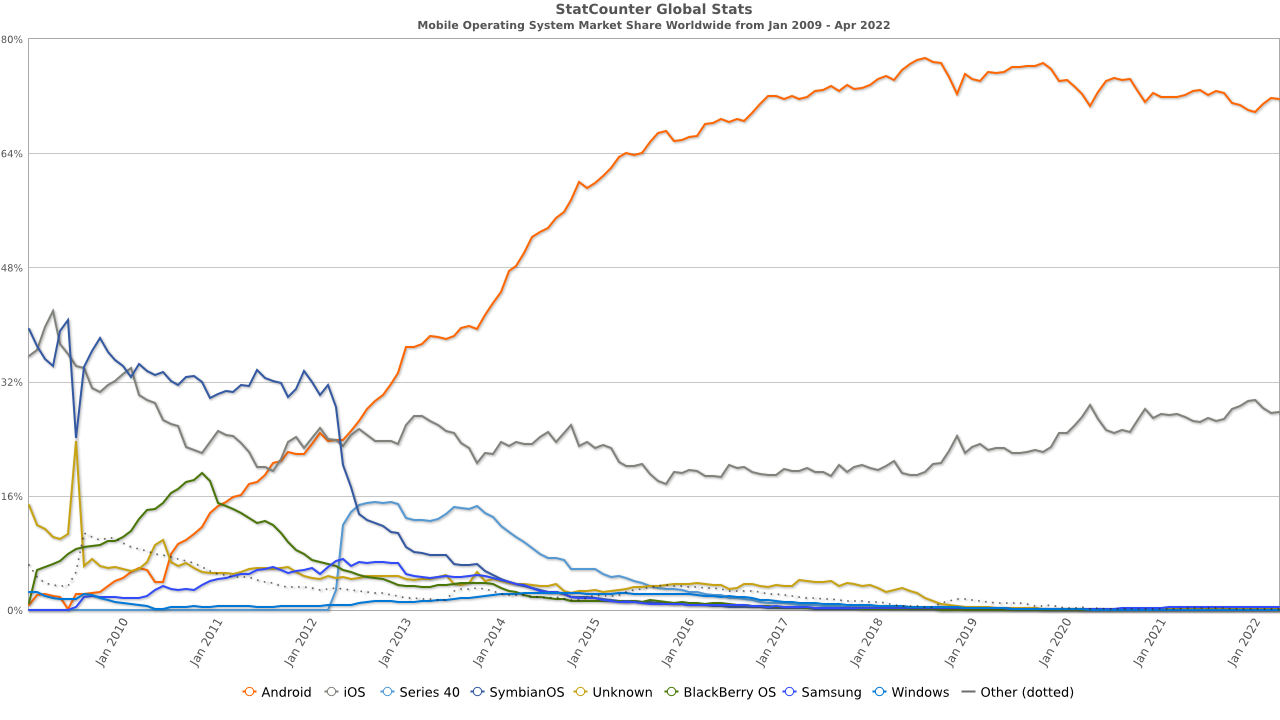
\includegraphics[scale=.45]{StatCounter-os_global.png}}
\label{fig}
\end{figure}
By giving more options to developers, their market share fell much slower than Symbian's did, and Blackberry was able to figure out new directions to take the company. As a result, the company is still alive, and has shifted their focus to cybersecurity. 

Having a central, unified app store is something that is crucial to a marketable smartphone, and something that Symbian suffered for not being prepared for. While there are currently debates on how harmful monopolies on app stores may be, there is no denying that having a central app store has been what has brought IOS and Android to the market domination that they command today. 

\subsection{Development}
\tab There is a clear shift to doing things more efficiently. In the past, developers swapped between many different frameworks, languages, and compatibility differences. This was the case with Symbian and having to develop for four different UI's. Nowadays, instead of typically having to develop for Symbian, BlackberryOS, SamsungOS, and others, developers only have to deal with IOS, Android, and/or web apps. Between these three platforms, their apps can be reached by the vast majority of devices. As seen with Blackberry and Apple, those who embrace these developer tools and cross-platform frameworks tend to do better as in the market.

Recently, apps are being built more often in cross-platform frameworks. This allows developers to code for multiple interfaces at once, saving development time and headaches. This greater efficiency does have correlation with the singularity of IOS and Android devices, although it is difficult to prove that it was caused solely because of this. However, there is a rise in React Native and Flutter usage, as 80\% of software developers say that they use at least one.\cite{vailshery_2022} These frameworks typically compile to IOS and Android, but not other mobile operation systems. Note that some also build to web applications, which often can be accessed by other mobile operating systems via a web browser. 

Development has also shifted to consider user experience in as many cases as possible. Hence, new testing technology has been developed. Besides having user testing websites and quality assurance testers, developers can also test their applications in virtual environments. These essentially simulate certain instances that a device may be in, allowing the app to be tested in a variety of different situations. For instance, Android Studio allows apps to be tested with various phone settings, including simulating slow internet connections. Independent developers have also created virtual environments that allow testers to bring their apps into a simulated space.\cite{vrtestbed} This gives unique opportunities such as being able to test the app in different lighting/times of day, or in spaces where there might be various sounds, such as in a coffee shop. This kind of growth in mobile application testing means that more real-world usable programs have come about as a result.

\subsection{Future Development}
\tab Development is changing quickly. Even over the last couple of years, IOS and Android have progressed to become almost exclusively the only two mobile operating systems in the global market. This means that cross-platform development apps are becoming more relevant for developers as they only have to develop for two ecosystems, both of which have a wide range of development tools. Most cross-platform development programs handle Android, IOS, and web apps. While React Native and Flutter dominate this sphere, there are also other technologies such as Unity which provides a suite of game development tools. The future seems to be with IOS and Android, but it is entirely possible their technology could become outdated just like Symbian and Blackberry became due to some unforeseen major improvement.

\subsection{Fringe operating systems}
\tab Although Android and IOS currently present as a duopoly, there are new operating systems being released. However, none have directly challenged this duopoly since their rise in 201. Still, many system's target markets make sense from a business perspective. For example, kaiOS is an lightweight operating system built for handsets, essentially turning T-9 phones into smartphones. They target first-time phone users in emerging markets. Their strategy seems to have worked, in May 2019 100 million handsets were running kaiOS.\cite{lunden_2019} In India, kaiOS overtook IOS from September 2018 to August 2019 to become the second-most prevalent operating system in India, peaking at almost 5\% of market share. However, it has slowly fallen since then and sits at 0.75\% of India's mobile OS market share.\cite{statcounter_india}
\begin{figure}[h]
\centerline{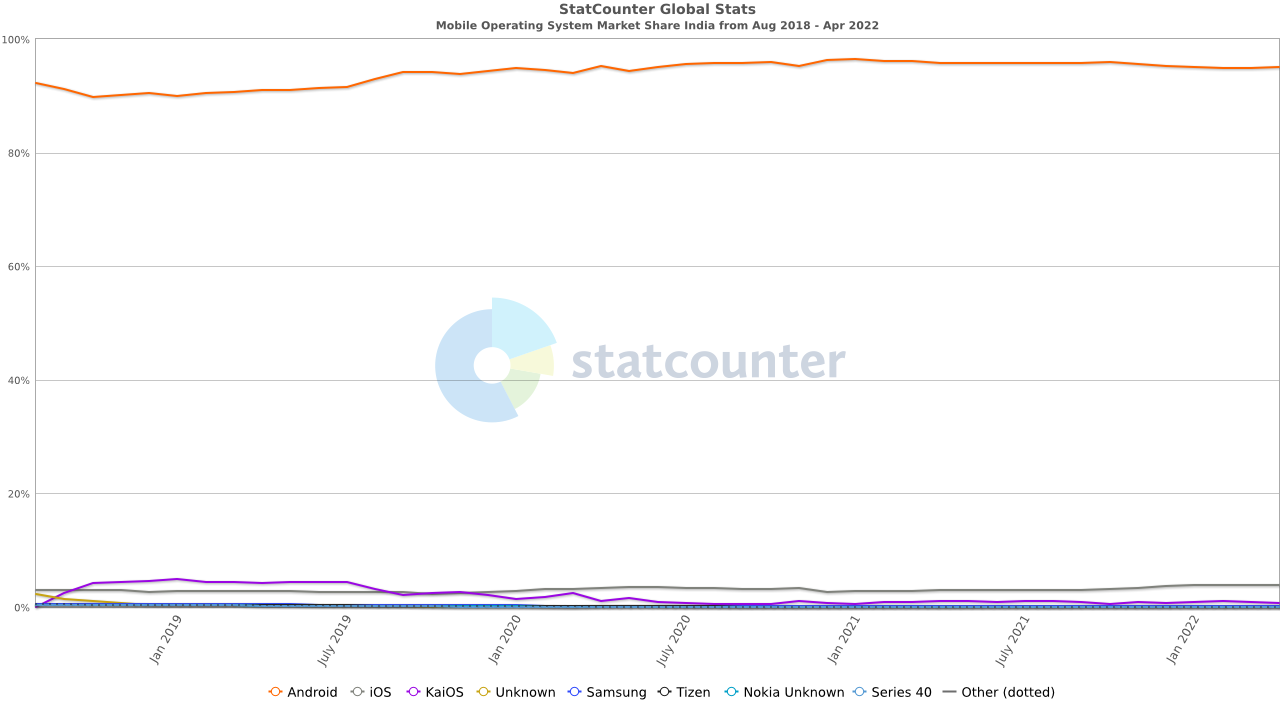
\includegraphics[scale=.45]{StatCounter-os_India.png}}
\label{fig}
\end{figure}
While these operating systems have not taken over the market, they are still successful businesses and have shown the potential to disrupt market leaders. As such, developers of mobile apps will likely need to keep an eye on emerging technology and markets as they present market opportunities. By 2020, there were over 800 kaiOS apps.\cite{vaghela_2021} While this is a healthy number, it could be argued that this is a miniscule number for a userbase including over a hundred million phones. If developers create for kaiOS, they are probability-wise more likely to have a breakthrough app than on Android or IOS app stores. As more niche markets arrive and grow, more niche operating systems will be created to serve them, something developers and companies should keep an eye on.

While there are some fringe operating systems that are built from the ground up, most developers find that their desired operating systems would work fine on current platforms. It is much more cost-efficient and easy to build off of current platforms, a feature which Android conveniently offers. This may be one of the reasons that no operating system has broken the grip that Android and IOS have had in the past few years, it is difficult and makes little sense to attempt the feat in the status quo. As Android is open-source, developers can make anywhere from minor changes to entire unique experiences by building on the platform.\cite{brown_2022} Thanks to the freedom given to developers, many fringe operating systems already have their base created for them. For instance, Lively's Jitterbug phones are designed for non tech-savvy seniors. Every aspect takes the user into consideration and thus the phone's interface looks vastly different from IOS or Android. However, the newest phone in the series, the smart3, is built off of Android 10.0.\cite{campisano_2021} Thanks to the presence of tools for developers and ease provided, many fringe operating systems are technically Android skins, and such will continue to assist Android's market influence rather than challenging it. This can serve as a counterargument to the idea that developers and companies should keep an eye on emerging tech for market opportunities. If Android's influence is going to continue expanding in these niche areas, the future of app development should continue to be focused on Android.

\subsection{Dark Patterns}
\tab Another way mobile apps may develop in the future surrounds dark patterns. Dark patterns are user interface aspects that intentionally confuse the user and get them to take actions they otherwise may not take. For instance, this could include putting a fake exit button on an advertisement. The user presses the exit button, but it still takes them to a download page to entice the user into downloading an app. According to a study, dark patterns are very prevalent. In a study of 240 popular apps, 95\% had dark patterns in their interfaces.\cite{darkpatternsandwheretofindthem} Dark patterns can exist in other ways as well. Social media apps that include systems that incentivise addiction are an impactful form of dark patterns, especially considering the current rise in tech addictions.\cite{pretz_2016} Attention has been called to these dark patterns, but there is a conflict of interest in tech companies between giving users free usage of programs versus collecting data and using it for business purposes. As tech companies figure out what responsibility they have towards the best interests of people versus the needs of the company, the issue of dark patterns will continue. The more dark patterns are brought into the spotlight and discussed, the more that companies will be cognizant of dark patterns in their design decisions. Thus, with continued accountability, there is a greater chance that harmful dark patterns will diminish in the future.

\section{Conclusions}
\tab The influence of mobile apps is undeniable. From the party tricks and helpful business assistance apps in IBM's SIMON, to the fall of Symbian, to the rise of IOS and Android's current market duopoly, mobile apps had a hand in all of it. Symbian's fall was due much in part due to the presence of better options on the market that had unified app stores. These better options were supported by the ease of development that mobile app creators had. Successful mobile operating systems have at least one core app market that has the trust of both developers and consumers. Cross-platform development follows market patterns, and many options help developers create for both Android and IOS. This ease of development has also supported Android and IOS's market dominance. The future is uncertain, but will certainly be influenced by which app markets can capture the trust of consumers and developers. Fringe operating systems have the potential to be successful businesses, but there are currently no serious contenders to become new global market leaders. The design of mobile apps can also be influenced by consumers. As discussed with dark patterns, if consumers are united in certain issues, such as dark patterns, they are more likely to be given attention by developers. However the uncertain future of mobile computing progresses, mobile applications will play a dominant role in their market influence.

\section{Future Research}
\tab The tech market develops and changes rapidly, and the next few years will be no exception. Just like Symbian and BlackberryOS were market leaders before they crashed spectacularly, Android and IOS cannot guarantee unshakable market dominance, no matter how secure they appear in the status quo. Thus, conducting similar research in five or ten years could create interesting comparisons to the state of mobile application's development process and market influence in 2022. This summary of mobile app's history is a helpful summary on which to base future research upon. Future research areas could include what is discussed here, such as dark patterns and cross-platform development, or it could expand to other untouched areas such as smartwatches or virtual/augmented reality apps. Wherever the topic is, there will always be more to learn of in this rapidly-changing field.


\bibliographystyle{plain}
\bibliography{bibliography.bib}

\end{document}
